\originalchapter{作业 5}
MIT 18.330, Spring 2012. 原件: Homework 5, Due Tuesday April 12. 整理注: 原印星期与 2012 年 4 月 12 日 (星期四) 不符, 此处保留原件信息. 以下解答均为 AI 编写, 非官方答案.

\begin{exercise}\label{ps5-q1}
(原题 1, 4 分) 考虑简谐振动初值问题
$y''+\omega^2y=0$, $y(0)=y_0$, $y'(0)=y_1$.
以下取 $y_0=0$, $y_1=1$, $\omega=1$.
\begin{enumerate}[label=(\alph*)]
\item 显式求解.
\item 引入 $z=y'$, 将其写成两个一阶方程组成的系统.
\item 用前向 Euler 法数值求解. 找出保证稳定的时间步长条件, 在 $(y,z)$ 平面画出解曲线.
\item 对后向 Euler 法回答同样问题.
\item 对梯形法回答同样问题.
\item (附加 1 分) 严格解释为何梯形法的点“恰好”落在单位圆上.
\end{enumerate}
\end{exercise}
\begin{solution}
(a) $y(t)=\sin t$.
(b) $Y=(y,z)^T$ 满足 $Y'=AY$, $A=\left(\begin{smallmatrix}0&1\\-1&0\end{smallmatrix}\right)$, $Y(0)=(0,1)^T$.
(c) 前向法 $Y_{n+1}=(I+hA)Y_n$, 两个放大因子为 $1\pm\ii h$, 模为 $\sqrt{1+h^2}>1$. 因此没有正步长能使无限时间迭代有界; 半径每步乘以 $\sqrt{1+h^2}$, 向外螺旋. 对固定有限时间, 当 $h\to0$ 仍收敛, 这与绝对稳定区的判断不同.
(d) 后向法 $Y_{n+1}=(I-hA)^{-1}Y_n$, 放大因子模为 $1/\sqrt{1+h^2}<1$, 任意 $h>0$ 稳定, 但有人工阻尼.
(e) 梯形法 $Y_{n+1}=QY_n$, $Q=(I-hA/2)^{-1}(I+hA/2)$, 放大因子 $(1\pm\ii h/2)/(1\mp\ii h/2)$ 的模等于 $1$, 任意 $h>0$ 稳定.
(f) $A^T=-A$, 且各矩阵均为 $A$ 的有理函数, 彼此交换. 因此 $Q^TQ=I$, 即精确算术下 $\|Y_n\|_2=1$. 浮点计算只能达到舍入误差范围内的保持, 不保证字面上的完全相等.
\begin{center}
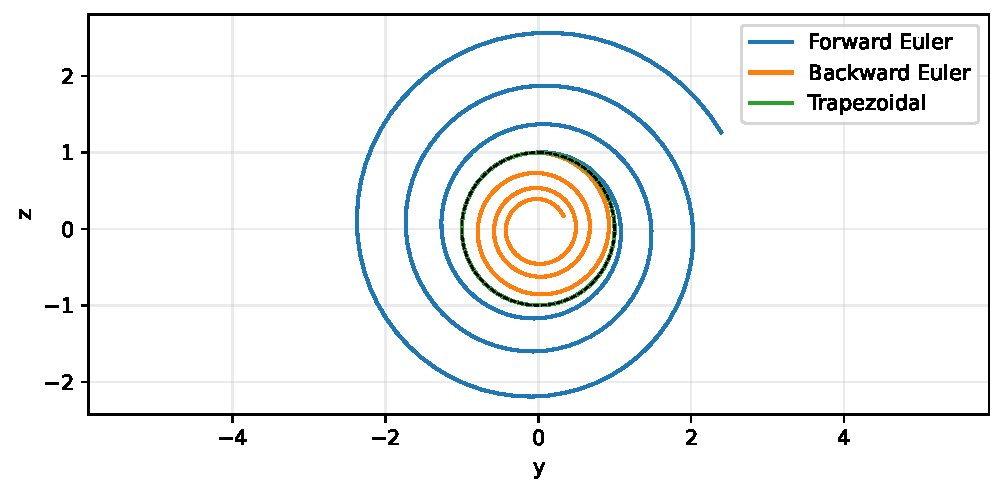
\includegraphics[width=.9\linewidth]{figures/assessments/ps5_phase.pdf}
\end{center}
实际取 $h=0.1$, 迭代 200 步; 前向、后向及梯形的最终半径分别为 $2.7048138294$, $0.3697112123$, $1.0000000000$. 梯形半径的最大偏差约 $8.3\times10^{-15}$.
\end{solution}

\begin{exercise}\label{ps5-q2}
(原题 2, 3 分) Leap-frog 法为
$y_{n+1}=y_{n-1}+2hf(t_n,y_n)$.
它是 $y'=f(t,y)$ 的最简单二步法. 求其在复数 $h\lambda$ 平面中的稳定区域.
\end{exercise}
\begin{solution}
对 $y'=\lambda y$, 设 $z=h\lambda$, 特征方程为
$r^2-2zr-1=0$. 两根的乘积为 $-1$, 若都在闭单位圆内, 则两根模都必须等于 $1$. 写 $r_1=\ee^{\ii\theta}$, 则 $r_2=-\ee^{-\ii\theta}$, 由和为 $2z$ 得 $z=\ii\sin\theta$. 因此只有虚轴线段可能稳定.
对 $z=\ii\eta$, $|\eta|<1$, 两根为
$\ii\eta\pm\sqrt{1-\eta^2}$, 模为 $1$ 且互异, 满足二步法根条件.
在端点 $\eta=\pm1$ 出现重根 $\pm\ii$, 通解含 $n(\pm\ii)^n$, 不稳定.
故按根条件稳定区域为 $\{\ii\eta: -1<\eta<1\}$, 包含 $0$, 没有二维内部. 若“绝对稳定”专指两根严格小于 $1$, 则该区域为空; 本题采用通常允许单位圆上单根的有界稳定定义.
\end{solution}

\begin{exercise}\label{ps5-q3}
(原题 3, 3 分) 考虑 $y'=-y^2$, $y(0)=100$, 真解为 $y(t)=1/(t+1/100)$.
\begin{enumerate}[label=(\alph*)]
\item 证明前向 Euler 迭代满足 $y_n\le100$.
\item 求保证前向 Euler 法稳定的步长条件, 并证明.
\item 对不同步长运行前向 Euler 法, 检查数值行为是否符合 (b) 的预期.
\item 再问 (原件再次标为 c)): 用显式法还是隐式法更好? 为什么?
\end{enumerate}
\end{exercise}
\begin{solution}
(a) $y_{n+1}=y_n-hy_n^2\le y_n$, 对任意 $h\ge0$ 归纳得 $y_n\le100$. 这个上界不保证下界或稳定.
(b) 若 $0<h\le1/100$, 则对 $0\le y_n\le100$,
$y_{n+1}=y_n(1-hy_n)\in[0,y_n]$, 所以解始终非负、有界; 在这一不变区间内迭代映射的导数 $1-2hy$ 属于 $[-1,1]$, 两条这样的轨迹之间的扰动不增长. 若 $h>1/100$, 首步变负. 写 $a_n=-y_n>0$, 后续有 $a_{n+1}=a_n+ha_n^2$. 若它有有限极限 $L$, 则 $L=L+hL^2$, 与 $L\ge a_1>0$ 矛盾, 故 $y_n\to-\infty$.
因此对给定初值, $0<h\le0.01$ 是轨迹有界的精确范围. 取等号时首步直接变成零, 虽有界却精度很差, 实用计算应取远小于 $0.01$ 的步长.

(c) 实验取 $h=0.005,0.01,0.015,0.02,0.021$. 前两者分别单调趋零、首步归零; 后三者首步为 $-50,-100,-110$, 随后发散, 与上述证明一致. 在真解附近仅考察 $|-2hy+1|\le1$ 并不足以保证数值轨迹留在真解的邻域.
\begin{center}
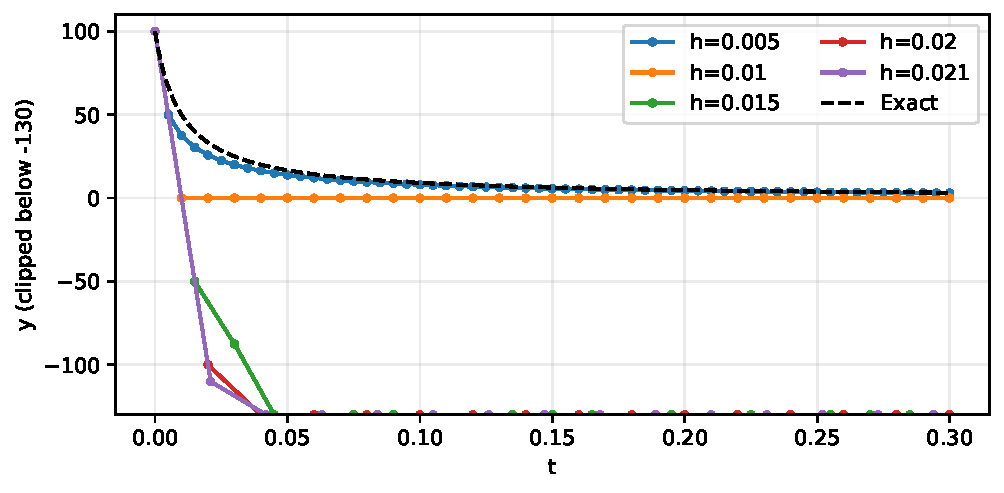
\includegraphics[width=.9\linewidth]{figures/assessments/ps5_nonlinear.pdf}
\end{center}
图对低于 $-130$ 的值作截断显示, 未将截断后的平台解释为稳定.

(原第二个 c)) 后向 Euler 满足 $hy_{n+1}^2+y_{n+1}-y_n=0$. 对非负 $y_n$ 选择正根, 用避免相消的形式
$y_{n+1}=2y_n/[1+\sqrt{1+4hy_n}]$,
任意 $h>0$ 都有 $0\le y_{n+1}\le y_n$, 且对输入的导数为
$1/(1+2hy_{n+1})\le1$. 隐式法允许较大步长而不出现负向爆破, 对稳定性更有利; 若要求准确解析初始快速变化, 两种法都仍需小步长或自适应. 本问题的隐式方程有显式正根公式, 每步代价也很小.
\end{solution}
